\documentclass{llncs}
\usepackage{graphicx}
\usepackage{color}
\usepackage{enumitem}
\usepackage{hyperref}
\usepackage{dirtytalk}
\usepackage[utf8]{inputenc}
\hypersetup{
    colorlinks=true,
    linkcolor=blue,
    filecolor=magenta,      
    urlcolor=cyan,
}
%%%%%%%%%%%%%%%%%%%%%%%%%%%%%%%%%%%%%%%%%%%%%%%%%%%%%%%%%%%%%%%%%%%%%%%%%%
\usepackage{todonotes} % use this to see the comments
%\usepackage[textsize=tiny]{todonotes} % use this to see SMALL : ) comments
%\usepackage[disable]{todonotes} % use this to hide all comments
%%%%%%%%%%%%%%%%%%%%%%%%%%%%%%%%%%%%%%%%%%%%%%%%%%%%%%%%%%%%%%%%%%%%%%%%%%


\newcommand{\todoinline}[1]{
    \todo[inline]{#1}
}
\newcommand{\todoiteminline}[3]{
    \todoitemtemplate{#1}{#2}{#3}{inline}{red}
}

\newcommand{\todoproofread}[3]{
    \todoitemtemplate{#1}{#2}{Please proof read above section; #3}{inline}{yellow}
}
\definecolor{mygreen}{HTML}{00CC00}
\newcommand{\todoproofreadDone}[3]{
    \todoitemtemplate{#1}{#2}{Please proof reading above section, done; #3}{inline}{mygreen}
}
\newcommand{\todoproofreaddone}[3]{
    \todoproofreadDone{#1}{#2}{#3}
}

\newcommand{\todoitemtemplate}[5]{%
% \index[MYTODO]{#2}
\todo[#4,color=#5,caption=X]{{#1}{ \textbf{{\tiny{for}} #2}:}{#3}}%
}

\newcommand{\todoiteminlinedone}[3]{
    \todoiteminlineDone{#1}{#2}{#3}
}
\newcommand{\todoiteminlineDone}[3]{
    \todoitemtemplate{{\commentsDoneFont{#1}}}{{\commentsDoneFont{#2}}}{{\commentsDoneFont{#3}}}{inline}{green}
}

\newcommand{\todoitem}[3]{
    \todoitemtemplate{#1}{#2}{#3}{}{red}
}
\newcommand{\todoitemdone}[3]{
    \todoitemDone{#1}{#2}{#3}
}
\newcommand{\todoitemDone}[3]{{\commentsDoneFont\todoitemtemplate{{\commentsDoneFont{#1}}}{{\commentsDoneFont{#2}}}{{\commentsDoneFont{#3}}}{}{green}}}


\begin{document}



%\title{All about Indexing for Question Answering systems: A deep dive into Information retrieval}
%\title{Graph vs RDF stores: An Empirical Evaluation of NoSQL RDF Data Management Solutions}
%\title{An Empirical Evaluation of NoSQL RDF Data Management Solutions}
%\title{Benchmarking RDF Data Management Solutions}
\title{LITMUS: An Open Extensible Framework for Benchmarking RDF Data Management Solutions}


\author{Harsh Thakkar\inst{1}, Mohnish Dubey\inst{1}, Gezim Sejdiu\inst{1}, Axel-Cyrille Ngonga Ngomo\inst{2}, Jens Lehmann\inst{1,3}, S\"{o}ren Auer\inst{1,3}\dots}
\institute{
	University of Bonn; \\
	\email{\{thakkar,dubey,sejdiu,jens.lehmann,auer\}@cs.uni-bonn.de}
	\and 
	University of Leipzig; \\
	\email{ngonga@informatik.uni-leipzig.de}
	\and 
	Fraunhofer IAIS;
\vspace{-10pt}
	}
\maketitle

\begin{abstract}

Developments in the context of Open, Big and Linked Data have led to an enormous growth of structured data. 
To keep up with the pace of efficient consumption and management of the data at this rate, many Data Management Solutions (DMS) have been developed for specific task and applications.
In this position paper, we present LITMUS,  \dots 
\todoiteminline{Harsh}{all}{Please contribute in the abstract writing}

\end{abstract}

\section{Introduction}\label{sec:Introduction}
     
    \todoiteminline{Harsh}{all}{This needs re-phrasing, please contribute for writing this}
    
Currently, we observe an enormous growth of structured data being made available on the Web as Open or Linked Data\footnote{http://lod-cloud.net/} as well as Big Data within organizations. 
With such a rapid growth in the amount of data, managing this data has also become a challenging issue. 
Modern day organizations face increasingly the need to search for data management tools, suited best for specific tasks. 
Choosing the best data management tool however is challenging and cumbersome due to the limited comparability and compatibility. 
With limited domain expertise and non-stop expansion of data the need for a standardised framework to benchmark and analyse the existing diverse data management landscape is of paramount importance.

Despite the growing interest and use in both research and industrial communities, current DMS benchmark creators do not offer a common cross domain suite for creating task specific benchmarks and there is no single baseline to compare one against the other. 
Moreover, re-producing or replicating benchmarks, created by others, is a non-trivial problem owing to reasons such as, non-standardised setup configurations, lack of publicly available resources (such as scripts, packages, etc) and lack of transparent evaluation policies. 
    %due to a variety of reasons including (i) unclear setup configuration, (ii) non-standard . as the unit of verification of the results for a whole systems. 
    %In order to fill the gaps (i) to help end user to choose the right system by showing the ranked results of the system's behaviors for the different parameter selection permutation, and (ii) the involvement of industry community to improve their systems by modeling a different challenges and pick a right pipeline for their needs.
    
There have been many research efforts in the direction of benchmarking a range of DMS, including some which have also considered evaluating cross domain DMS {cite graphium, pandora}, but only to a limited scope. \todo[color=green]{Harsh: working on this, Need to add more information here..}
    
    
In this paper we present LITMUS, an open extensible approach for benchmarking a wide variety of NoSQL Data Management Solutions (DMS). 
LITMUS aims to support organizations which aspire to use Linked Data management technologies in a wide spectrum of applications and magnitudes. 
LITMUS will provide realistic performance evaluation platform covering a plethora of heterogeneous technologies (see Section~\ref{litmus_framework}) for storage and querying benchmarking. 
\todoproofread{Sören}{Harsh}{Add more details in 2-3 sentences about the LITMUS approach}

To put the reader in to the context of this work, we present the following \textbf{user scenario}: 
    
    \say{Harsh (say) works in a research project called WDAqua\footnote{WDAqua ITN - wdaqua.informatik.uni-bonn.de}. WDAqua aims towards building a data-driven question answering by using web data (which is available in various formats e.g. RDF, CSV, SQL, XML, etc). Harsh is responsible for ensuring efficient data management (storage and retrieval) for this project. There is an ocean of data management tools, each deliberately tailored for handling specific format of data, which use a wide variety of indexing, storage and query representation mechanisms. \textit{Harsh wants wants to assess the performance (benchmark) of these DMS against each other (for a varying degree of factors such as the query typology, indexing speed, index size, query response time, etc) and choose the best solution for his needs}. However, benchmarking is a task which demands tedious manual efforts, owing to the diversity in the nature of these DMS and the granularity of the repetitiveness involved within. 
    %The major reasons for this diversity is that each of these DMSs represent queries in a different language, employ a spectrum of indexing and storage mechanisms, etc.  
    \textit{Harsh wants to automatise the whole benchmarking process of these cross domain DMSs, allowing easy integration, evaluation on custom loads, and fast analysis of the evaluation results}. He would also \textit{expect the framework to be flexible to integrate new DMSs to the plethora of existing systems and benchmark them against a baseline}. The answer to Harsh's questions is \textbf{LITMUS}. LITMUS is an open extensible platform for benchmarking cross-domain DMSs. LITMUS, will not only satisfy Harsh’s need for automatising the tedious benchmarking process, but also offer: \textit{\textbf{(1)}} an efficient way for replicating existing benchmarks (such as BSBM\cite{bizer2009berlin}, WAT-DIV\cite{alucc2014diversified}, etc), \textit{\textbf{(2)}} a wide set of performance evaluation measures/indicators tailored specifically keeping in mind the DMSs being benchmarked, and \textit{\textbf{(3)}} visualising the performance comparison of the DMSs on various intrinsic factors via custom charts, graphs and tabular data allowing easier and faster insight.}
    \todoproofread{Harsh}{Maria}{}
    
    %The objectives of LITMUS are to:\todo[color=green]{Harsh@all: Do we need the objectives now? after having presented the user scenario}
     %\begin{itemize}[nosep]
      %  \item provide a open extensible platform to benchmark, compare and analyse cross domain DMSs with respect to a wide variety of data and queries;       
       % \item to automatise the benchmarking phenomenon allowing easy replication, integration and evaluation of existing third party benchmarks to an existing plethora of tools;
    %    \item explore and study a wide range of storage and indexing techniques used by existing DMS and their correlation with a wide spectrum of performance indicators
     % \end{itemize}
    
The remainder of this article is organised as follows: 
We briefly present a survey of existing benchmarking efforts and their shortcomings in Section~\ref{relwork}. 
Then in Section~\ref{Objectives}, we shed light on the focus of LITMUS, the challenges to be addressed and the target communities which can benefit from LITMUS. 
We present the LITMUS framework and describe the components in brief in Section~\ref{litmus_framework}.  



%========================================RELATED WORK======================================
\section{Related work}\label{relwork}

Benchmarking is widely used for evaluating data stores. 
Benchmarks exist for a variety of levels of abstraction from simple data models to graphs and triple stores or even entire enterprise systems.
We describe the current state of the art in benchmarking, in particular benchmarks for (a) Relational databases, (b) Graph databases, (c) RDF stores, (d) Key-Value stores, (e) Wide Column stores and (f) Cross domain benchmarking efforts.
We identify shortcomings and limitations of existing systems in order to employ LITMUS by extending these benchmarks to deal with the challenges forced by new systems.
In addition to surveying existing work, we intend to focus mainly on the purpose and scope of the benchmarks.
    
    %Relational databases have standard benchmark suites such as TPC~\cite{Nambiar2011} for dealing with transaction processing, querying performance, data maintenance and other operations for a relational database.
    %The TPC~\cite{Nambiar2011} benchmark suit deals with transaction processing, querying performance, data maintenance and other operations for a relational database.
    In the context of \textit{Relational} DMSs there exists some well-established benchmarks, especially the well known plethora of Transaction Processing Performance Council (\textbf{TPC})~\cite{Nambiar2011} benchmarks.
    TPC benchmarks use discrete metrics for measuring the performance of the relational DMS. The online transaction processing benchmarks \textbf{TPC-C} and \textbf{TPC-E} use transactions per minute metric. The analytics benchmarks \textbf{TPC-H} and decision support benchmarks \textbf{TPC-DS} use the queries per hour at size and cost (in USD) per performance metrics.
    
    For benchmarking \textit{Graph} DMS, there are some existing works in their early stages (such as HPC Scalable Graph Analysis Benchmark~\cite{Dominguez-Sal:2010:SGD:1927585.1927590}, Graph 500~\cite{murphy2010introducing}, XGDBench~\cite{conf/cloudcom/DayarathnaS12}) dealing with graph suitability and graph analysis. However they fail on defining standards for graph modeling and query languages.
    
    %Existing RDF benchmarks have several limitations, mainly because they do not provide a comparison between a wide variety of DMS. However, 
    The substantial increase in the number of applications that use RDF data, has advocated the need for a huge scale benchmarking effort on all aspects of RDF Data life cycle mostly focusing on query processing\cite{ngomo2016hobbit}.
    RDF DMS benchmarks make use of real (i.e. DBPedia, Wikidata, etc) and synthetic (i.e. Berlin SPARQL Benchmark, WAT-DIV, etc) datasets, to evaluate DMS performance over custom stress-loads and setup environments\footnote{https://www.w3.org/wiki/RdfStoreBenchmarking}.
    DBPedia SPARQL Benchmark \textbf{(DBPSB)}~\cite{Morsey2011}, which uses real data, assesses RDF DMSs performance over DBPedia by creating a query workload derived from the DBPedia query logs. Basically, the process is based on mining the query logs, creating clusters and analyzing the features of the SPARQL queries that were most frequently used. The benchmark covers most of the SPARQL 1.0 language features such as (union, optional,join) and distinct, filter conditions and operators. However, it does not consider more complex language features such as inference or decision support queries.
    The Lehigh University Benchmark (\textbf{LUBM})~\cite{Guo:2005:LBO:1741305.1741322} is intended to evaluate the performance of Semantic Web repositories over a large synthetic dataset that comply to a university domain ontology.
    The LUBM benchmark consist mainly some lookup and join queries, and not considering complex SPARQL 1.0 operations (optional, union) or even complex reasoning and inference.
    The Berlin SPARQL Benchmark (\textbf{BSBM})~\cite{Bizer2009TheBS}, is another synthetic data based benchmark, which consists of e-commerce use case built around a set of products that are offered by different vendors.
    The BSBM benchmark provides of a data generator, which can be used to create sets of connected triples of any particular size, as well as a set of queries that measure the performance of RDF engines for very large datasets but not taking on consideration the ability of RDF engines to perform complex reasoning task.
    Waterloo SPARQL Diversity TEST Suite (\textbf{WatDiv})~\cite{alucc2014diversified} as, in contrast to other existing benchmarks, its main focus is to benchmark systems against varying query shapes to identify their weaknesses and strengths.
    Its model combines an e-commerce scenario with a kind of social network.
    WatDiv comes with a set of 20 predefined queries (star, linear, snowflake and complex). 
    One of the most commonly used synthetic data based benchmark is \textbf{SP2Bench}~\cite{books/sp/virgilio09/SchmidtHMPL09}. Like BSBM and WAT-DIV, it also contains a data generator and a set of queries. SP2Bench uses DBLP\footnote{http://dblp.uni-trier.de/db/} bibliographic schema to generate arbitrarily large datasets and consist of fourteen queries which employ different SPARQL 1.0 operators (optional, union, filter, orderby, etc) but do not support reasoning tasks.
   
    
    There are only a few efforts, countable on finger tips, which benchmark \textit{cross domain} DMS. \textbf{Pandora}\footnote{http://pandora.ldc.usb.ve/}, one such work, employs the Berlin SPARQL Benchmark data to compare RDF stores against Relational stores (Jena-TDB, Monetdb, GH-RDF-3X, PostgreSQL, 4Store). 
    \textbf{Graphium}~\cite{flores2013graphium} is a similar study benchmarking RDF stores against Graph stores (Neo4J, Sparksee/DEX, HypergraphDB, RDF-3X) on graph datasets including a 10M triple graph data generated using the Berlin SPARQL Benchmark data generator. Recently, the ongoing work at \textbf{LDBC}~\cite{DBLP:journals/sigmod/AnglesBLF0ENMKT14} focuses on combining industry-strength benchmarks for graph and RDF data management systems.
    The LDBC introduces a new bottleneck methodology for developing benchmark workloads, which try to combine user input with feedback's from systems experts.%\todo[color=green]{Gezim: @Harsh, please could you polish it for me and  make it clear that we do not want to involve any expert systems architects to do a cross-domain benchmarking?}
    
    The process of benchmarking DMSs is non-trivial, mostly due to the large amount of tedious human effort required for designing, administering, evaluating, and analysing the diverse nature of systems involved. The literature, until now, is more focused on benchmarking domain specific DMS, despite the need for integrating cross domain DMSs and automatising the tedious benchmarking process. LITMUS, is focused towards addressing these shortcomings  and serve as a open extensible platform to allow easy integration, benchmarking and analysis for the performance of a plethora of DMSs. There exist no such open, extensible and reusable framework exists to the best of our knowledge which allows to explore, analyse and play with such a wide range of DMSs.
    Our aim is to satisfy these criteria by developing a benchmark platform to serving systems, portable to different end data structure representation through our extensible framework, scalable to large scale data sets, and employing formal operations on top of it.
    
    
    %\todoproofread{Gezim, Harsh}{all}{and Review too. This needs a polishing and possibly shortening of text}

    
   % \begin{itemize}
   %     \item survey papers and other formal publications on benchmarking different graph stores, comparison of various triple stores and so on
    %    \href{https://docs.google.com/document/d/1DbtHvE4oaSuusPjeM2nGNBzrRArQt_rlCh3J5g2aIAE/edit?usp=sharing}{Literature review of Related Work}
        
    %    \item Papers on data, queries and other tools used for benchmarking
%    \end{itemize}
    
    
   % {\color{red}{Other benchmarks, Other such frameworks? LDBC council work to be cited Gerbil to be cited BAT-framework to be cited }}

\section{Objectives, Challenges and Outcomes}\label{Objectives}
    \subsection{Focus of the LITMUS framework}
        The LITMUS framework aims at bridging the gaps in adopting, deploying and scaling the consumption of Big Linked Data. LITMUS is being built with a dedication to simplify the use, assessment and analysis of the performances of a wide spectrum of Linked Data management solutions for satisfying the end user's needs.  In particular, the LITMUS project will create: (i) A common ground for carrying out benchmarks for a plethora of cross domain DMSs (ii) Specific benchmarks for the selected DMSs (in the later phases), and  (iii) Reports and scientific studies on the correlation of a variety of factors (\textit{such as} query typology, data structures used for indexing, etc) with the performances of the DMSs. The LITMUS framework will also, during its final phase, be able to serve as a recommendation medium for suggesting particular DMSs for the user specific setting or application based on predefined requirements. 
    \subsection{Challenges to be addressed}\label{challenges}
        In order to develop such an open extensible benchmarking platform (LITMUS), there are three key challenges which have to be addressed. We describe them in brief as follows:
        \begin{itemize}[nosep]
            \item \framebox[1.1\width]{\textbf{C1}} \textbf{Data conversion}: This challenge demands a generic data conversion mechanism. This will allow the user to convert the input data to a format interpretable by the corresponding DMS (e.g. RDF to CSV (Comma Separated Value), JSON (JavaScript Object Notation),  and SQL (Structured Query Language).
            \item \framebox[1.1\width]{\textbf{C2}} \textbf{Query Conversion:} 
            One of the substantial research gap is the language (query language) barrier. Since all query languages are different in a their structure and expressivity, and the DMS have different query languages, there is a need to develop an intermediate mechanism to convert or express the logic of one query (from SPARQL) to the other respective language (\textit{say} CYPHER, SQL, CQL, etc). For instance, path queries (in SPARQL) cannot be expressed in an equivalent manner in SQL. This requires an exhaustive study of the expressivity of query languages and a formal analysis of how they can be mapped to other languages without altering the meaning of the query. This study will provide us with deep insights about the functionality of various query languages, their strengths and limitations.
            also propose a solution approach in the block diagram (as mentioned above).
            \item \framebox[1.1\width]{\textbf{C3}} \textbf{Performance measures/indicators:} 
            The performance of a DMS can be assessed on a wide variety of metrics/features/indicators. It is necessary in order to conduct a correlation analysis of the impact of the diversity in queries and data on storage and indexing efficiency of the DMS. Apart from the traditional performance measures such as precision, recall, index size, storage size, number of triples, query response time, etc there is a need to explore more complex indicators of performance to successfully determine their correlation with the type of data and queries.
        \end{itemize}
    
    \subsection{Outcomes of LITMUS}
    The artifacts produced by the research and development activity for the LITMUS project can be grouped into two groups: \textit{(A1)} scientific studies and \textit{(A2)} framework/software. 
    
    \framebox[1.1\width]{\textbf{A1}}\textit{Scientific studies:} 
        \begin{itemize}[nosep]
            \item An in-depth analysis of the query language expressivity and supported features addressing the language barrier \textbf{(C2)} (ref. section \ref{challenges})
            \item An exhaustive exploratory study on the selection of performance measures/indicators for evaluating cross domain DMSs addressing challenge \textbf{(C3)} (ref. section \ref{challenges})
            %On top of the existing performance evaluation measures, we will study and analyse a series of other features such as the design of indexes and corresponding data structures on the retrieval performance for structured data. A detailed examination of the correlation between query typology and data storage and retrieval mechanisms.
        \end{itemize}
        
        \framebox[1.1\width]{\textbf{A2}} \textit{Framework/Software (i.e. algorithm(s), tools, etc):} 
        \begin{itemize}[nosep]
            \item An automatic mechanism for converting RDF data to multiple data formats on the fly (such as CSV, JSON, SQL, etc), enabling compatible data input for cross domain DMSs. 
            \item A novel automatic SPARQL to any query language converter enabling compatible query input for cross domain DMSs.
            \item An API allowing easy integration and deployment of third party DMSs for benchmarking in LITMUS
            \item An open extensible benchmarking platform, LITMUS, for cross domain DMS performance evaluation.
               % \todoproofread{Harsh}{all}{and Review too}

    \subsection{Target audience}
        \begin{itemize}[nosep]
            \item \textbf{Technology Vendors:}
            This addresses the Industrial/Commercial DMS developer fraternity (such as system and data analysts, system developers, system architects) who thrive towards developing more and more advanced DMS for an efficient consumption of BIG data.
            \item \textbf{Technology Consumers:}
            The users (personnel from the private and commercial organisations, associations, etc) seeking recommendation for the best solution for their needs can simply compare a wide range of DMS against a spectrum of desired parameters (types of queries, data, performance indicators) and choose the optimal one for their needs. 
            \item \textbf{Technology Researchers:}
            This includes the researchers who can benefit by absorbing the knowledge and contributing to the rigorous research efforts to for the research community. The target research audience will be the communities, not limited to Semantic Web, Database, Information Retrieval, Big Data researchers, etc.
        \end{itemize}
        %\todoproofread{Harsh}{all}{and Review too}


%========================================THE BENCHMARK FRAMEWORK======================================
\section{The Litmus Framework}\label{litmus_framework}
   % \subsection{Objectives}
   %    \todoinline{Needs to formulated well, suggest changes} 
   %   Why are we doing this? - To develop an Open, Extensible and Reusable cross domain platform for:
   %  \begin{itemize}
   %     \item Benchmarking data management solutions across a wide variety of categories
   %    \item Exploring and studying a wide range of storage and indexing techniques and their correlation with different types of queries and data
   %   \item Allowing easy integration and benchmarking of new third party data management solutions to an existing plethora of tools
   %   \end{itemize}
        

    \subsection{Architecture Overview}
        The LITMUS architecture comprises of four major facets or components: Data Facet (F1), Query Facet (F2), System Facet (F3) and the Benchmarking core (F4). Figure \ref{fig:benchmark_arch} illustrates the abstract workflow of the LITMUS framework. We now explain the role of each facet. 
         
        \begin{figure}[h]
            \centering
            %\includegraphics{}
            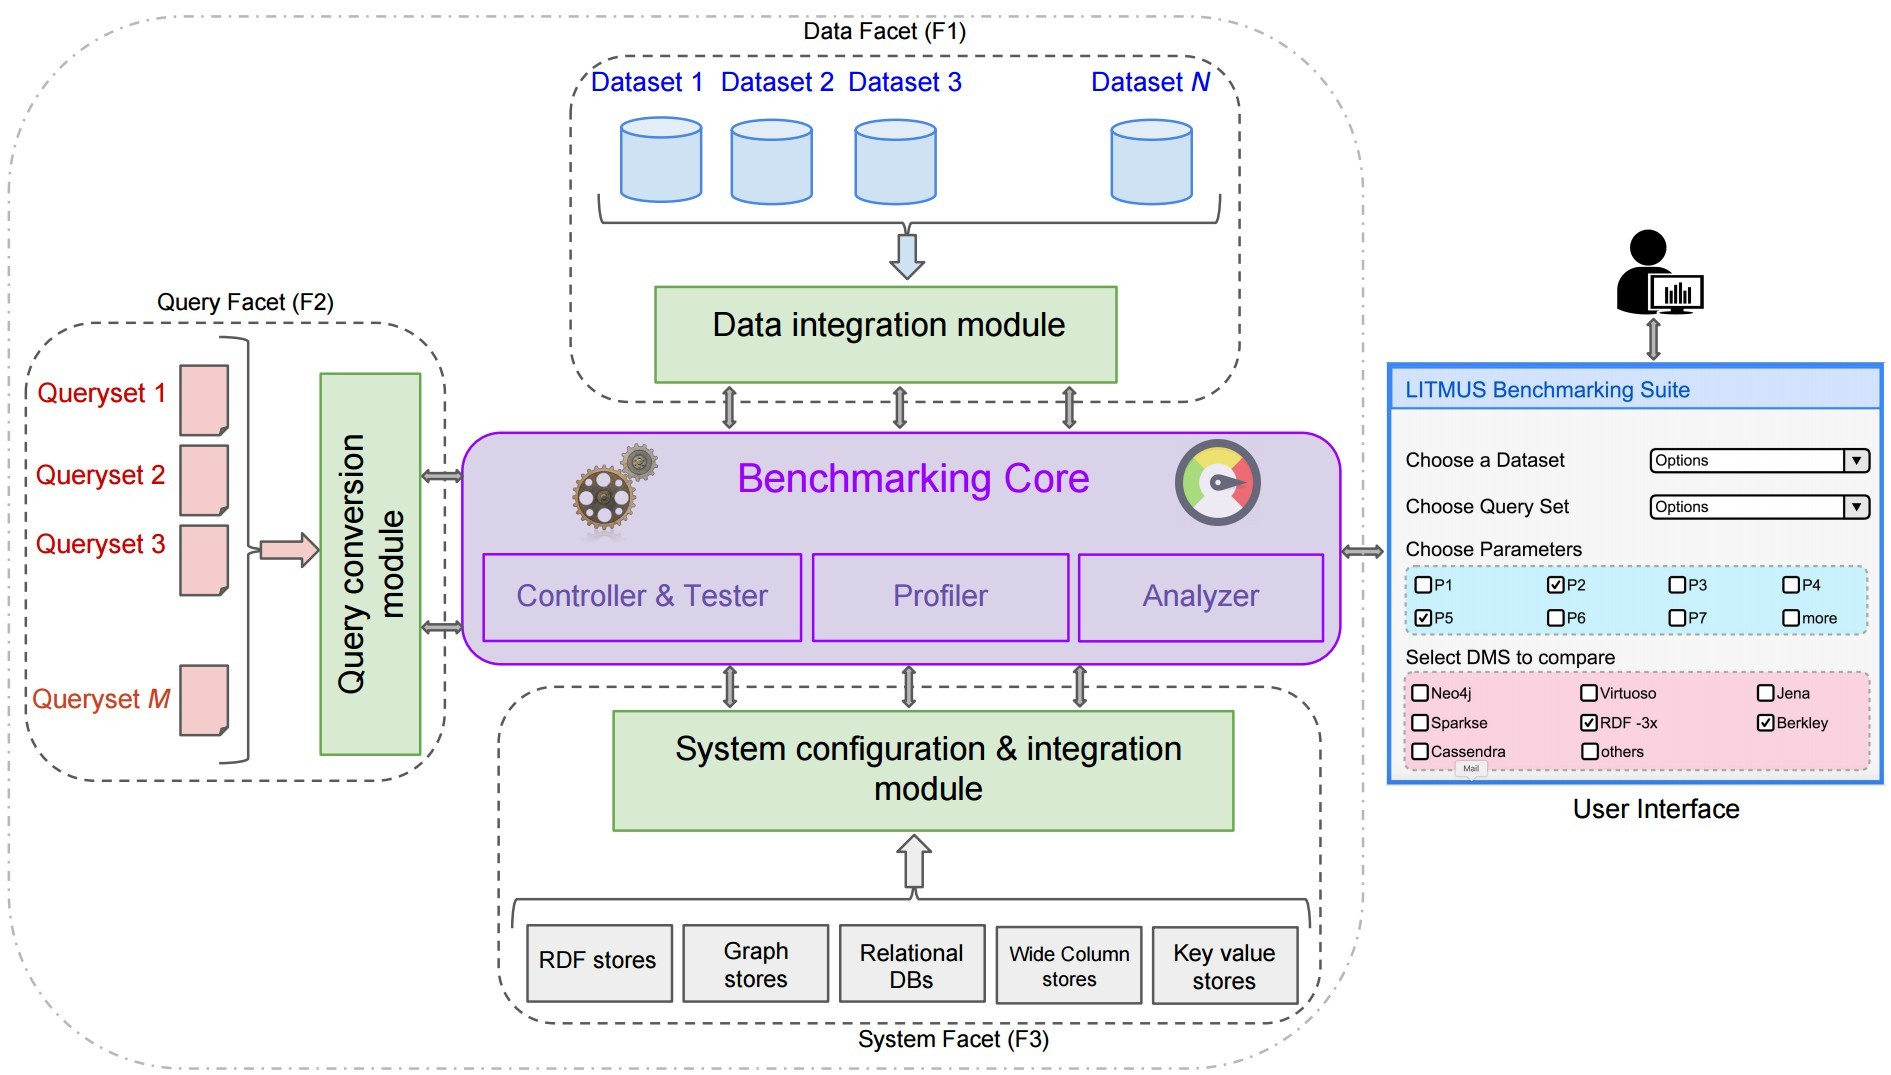
\includegraphics[scale=0.18]{images/benchmark_arch_latest_new}
            \caption{Overview of the LITMUS framework architecture.}
            \label{fig:benchmark_arch}
        \end{figure}
        
        \textbf{Data Facet \framebox[1.1\width]{F1}:} The Data Facet consists of two modules, \textit{(i)} Dataset(s) and \textit{(ii)} Data Integration Module. The \textit{dataset(s)} are the datasets chosen for benchmarking. These may be, real datasets such as DBpedia\footnote{http://wiki.dbpedia.org/}, Wikidata\footnote{https://www.wikidata.org}, etc or synthetic datasets such as the Berlin SPARQL Benchmarking (BSBM)~\cite{bizer2008benchmarking,bizer2009berlin}, Waterloo SPARQL Diversity Test Suite (WatDiv)~\cite{alucc2014diversified}, etc or hybrid datasets which comprise of both real and synthetic data. 
        The \textit{Data Integration Module}, one of the key contributions of the framework, is responsible for (a) making the data available to the system in requested formats (such as .NT, CSV, SQL, JSON) by carrying out appropriate data conversion and mapping tasks (i.e. Challenge \textbf{C1}), and (b) loading the desired format of data to the respective DMSs selected for the benchmark. 
        
        \textbf{Query Facet \framebox[1.1\width]{F2}:} The Query Facet consists of two modules. (i) Queryset(s), and (ii) The Query Conversion Module. The \textit{Queryset} refers to the set of query input files. The input queries are in SPARQL. The \textit{Query Conversion Module} will also be one of the key components of the LITMUS framework addressing the language barrier (Challenge \textbf{C2}). This module is responsible for: (i) converting the input SPARQL queries to respective DMSs query language (for instance, SQL, CYPHER, CQL, etc). The conversion will be performed using a state-of-the-art algorithm/technique which involves an intermediate language representation form. Thus, the \textit{Query Conversion Module} module will allow a wide variety of SPARQL queries (such as path, star-shaped and snowflake queries) to be converted into a wide variety of query languages, ultimately solving the language barrier.
        
        \textbf{System Facet \framebox[1.1\width]{F3}:} The System Facet, like the previous facets, also consists of two key modules, (i) DMSs and (ii) DMS Configuration and Integration module. The \textit{DMSs} module  constitutes of the DMS selected for the benchmark. The \textit{DMS Configuration and Integration} module is responsible for (i) providing easy integration via wrapper(s) or as a plugin of the DMS to the end user, (ii) Monitor and configure the the integrated DMS for the benchmark. On top of this, this module will make use \textit{dockers} for ensuring a fair allocation of resources and necessary isolation required for conducting realistic benchmarks. 
        
        \textbf{Benchmarking core \framebox[1.1\width]{F4}:} The Benchmarking core (aka LITMUS core) is the heart of the LITMUS framework, consisting of three modules (i) Controller and Tester, (ii) Profiler, and (iii) Analyser. The \textit{Controller and Tester} is responsible for executing the respective scripts for: loading the data and queries to their corresponding DMSs, creating and validating the specified system configurations, and finally executing the benchmark on the selected setting. The \textit{Profiler} is responsible for: (a) generation and loading of various profiles (stress loads, query variations, etc) for conducting the benchmark tests and (b) writing the benchmark results profile-wise to the files (disk). The \textit{Analyser} is responsible for the collection of the results of the benchmark from the \textit{Profiler} and generates the performance evaluation reports. It also carries out the correlation analysis between the aforementioned  parameters by the user. The final results (reports) are then presented to the end user in a suitable visualization format (such as plots, tables, charts etc)
        %\todoproofread{Harsh}{all}{and Review too}
    
    
%\section{NoSQL Data management systems}
%\todoiteminline{Harsh}{all}{I propose we merge this in the motivation, making it an independent section rather than a subsection. We have to focus on why we are proposing such a framework. Mentioning these diverse systems will only strengthen our claims}

  
 %   RDF stores
    %\subsubsection{Jena}
    %\subsubsection{Sesame}
    %\subsubsection{4store}
    %\subsubsection{Redland}
    %\subsubsection{Strabon}
    %\subsubsection{BrightstarDB}
    %\subsubsection{\color{red}{system... n}}
    
  %  Graph stores
    %\subsubsection{Neo4J}
    %\subsubsection{Titan}
    %\subsubsection{Giraph}
    %\subsubsection{InfiniteGraph}
    %\subsubsection{FlockDB}
    %\subsubsection{Sparksee}
    %\subsubsection{\color{blue}{system... m}}
    
    %\subsection{Multi-model stores}
    %\subsubsection{\color{green}{system... o}}
    
   % Key-Value stores
    %\subsubsection{K-V store 1}
    %\subsubsection{K-V store 2}
    
%    Wide Column stores
    %\subsubsection{W-C store 1}
    %\subsubsection{W-C store... r}
    
 %   Document-oriented stores
    %\subsubsection{D-O store 1}
    %\subsubsection{D-O store 2}





%========================================EVALUATION======================================
%\section{Evaluation parameters}
 %   \todoiteminline{Harsh}{co-authors}{Since we mentioned that we plan to produce a study of a wide range of performance indicators in sec 3.4, I propose we can just leave this for now with a small summary table of metrics used these days. or we can just skip this section all at once.}
  %  \subsection{Evaluation parameters}
   % System n VS m VS o VS p VS r VS s 
    
    
%\section{Case study?, User scenario?}
%\todoinline{do we need one?}

  
\section*{Acknowledgments}\label{sec:Acknowledgments}
The parts of this work are supported by funding received from the European Union's Horizon 2020 research and innovation program under the Marie Sklodowska-Curie grant agreement No 642795 (WDAqua ITN).

\bibliographystyle{abbrv}
\bibliography{ref}

\end{document}

